\subsection{Evaluation}
With the advancement of Large Language Models (LLMs), the performance of models in complex document processing and Retrieval-Augmented Generation (RAG) tasks has become a central focus of research.


\subsubsection{Visual Document Understanding and Basic QA Evaluation}

\begin{figure*}[t]
    \centering
    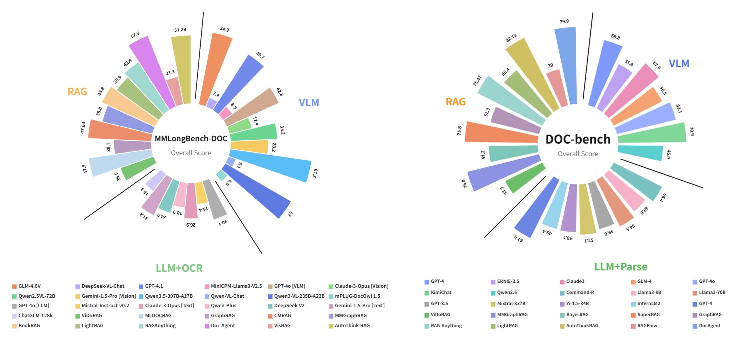
\includegraphics[page=1,width=\textwidth]{figs_by_qixingyu/fig09.pdf}
    \caption{Performance comparison of representative models on MMLongBench-Doc and DocBench, two benchmarks for evaluating multimodal long-document understanding.}
    \label{fig:combined}
\end{figure*}
Document Question Answering (DocQA) research primarily focuses on whether models can correctly understand text, layout, and visual cues from single-page or small-scale documents. DocVQA~\cite{docvqa2020} is one of the earliest benchmarks to systematically propose "question answering on document images," emphasizing the localization of facts by understanding text, layout, and visual cues in single-page documents. Document Collection VQA~\cite{doccollectionvqa2021} for the first time placed questions in a document collection scenario, requiring models to locate answers across multiple documents. InfographicVQA~\cite{infographicvqa2021} focuses on infographic QA to evaluate the model's understanding and reasoning capabilities in mixed scenarios of complex layouts, charts, and text. A Dataset of Information-Seeking Questions and Answers Anchored in Research Papers~\cite{infoseekqa2021} proposed a QA dataset oriented toward long scientific research papers, focusing on the types of questions readers actually ask while reading. DUE: End-to-End Document Understanding Benchmark~\cite{due2021} proposed a comprehensive benchmark for end-to-end document understanding, where models start from raw documents, obtain text and layout through OCR and layout modeling, and then complete downstream tasks. These datasets primarily focus on visual text understanding, region localization, and factual QA in single documents or small-scale collections, laying the most fundamental input and evaluation paradigm for subsequent "Retrieval + Reasoning."

Next, the research focus began to shift from "understanding one page" to "cross-page understanding and localization." Hierarchical Multimodal Transformers for Multi-Page DocVQA \cite{tito2023hierarchicalmultimodaltransformersmultipage} was the first to systematically handle multi-page documents, answering "what to do when information is scattered across multiple pages" through hierarchical structural modeling of pages and document-level semantics. VRDU~\cite{vrdu2023} proposed a "Visually Rich Document Understanding" benchmark and evaluation framework specifically for complex business document information extraction tasks in real business scenarios. Test-Time Adaptation for Visual Document Understanding~\cite{tta-vdu2023} is oriented toward visual document understanding, enabling models to adapt to new documents at test time.

Simultaneously, datasets with the problem setting of "locating evidence from a large number of pages" began to emerge. PDFVQA~\cite{pdfvqa2023} introduced real PDF documents into evaluation for the first time, where questions often require locating key information among many pages. SlideVQA~\cite{slidevqa2023} is a DocVQA dataset for multi-page slide documents consisting of slide images and natural language questions, used to study understanding and reasoning across multiple image pages. DUDE~\cite{dude2023} is a document understanding benchmark and evaluation framework proposed in 2023, oriented toward DocVQA and comprehensive document understanding evaluation on visually rich documents. DLUE \cite{dlue2023} is a comprehensive evaluation dataset and task suite for long and complex-structured documents, used to systematically assess model capabilities in document-level language understanding. KNVQA \cite{knvqa2023} proposed a knowledge-based visual QA evaluation dataset and benchmark, primarily used to assess the "factuality" and knowledge reasoning abilities of Large Vision-Language Models (LVLMs). Privacy-Aware Document VQA \cite{privacydocvqa2023} is a privacy-sensitive dataset and benchmark for DocVQA, used to study automatic QA and information extraction on real invoices under Federated Learning and Differential Privacy constraints, revealing the constraints of DocQA in real-world applications and pushing evaluation from ideal to reality. PDFTriage \cite{saad2024pdftriage} is a QA benchmark and methodology for long structured documents (e.g., PDFs), used to evaluate and enhance the QA capabilities of large models in "whole book / ultra-long context" scenarios, with a particular emphasis on the role of document structure (chapters, page numbers, tables, images, etc.) in retrieval and answering.

\begin{figure*}[t]
\centering
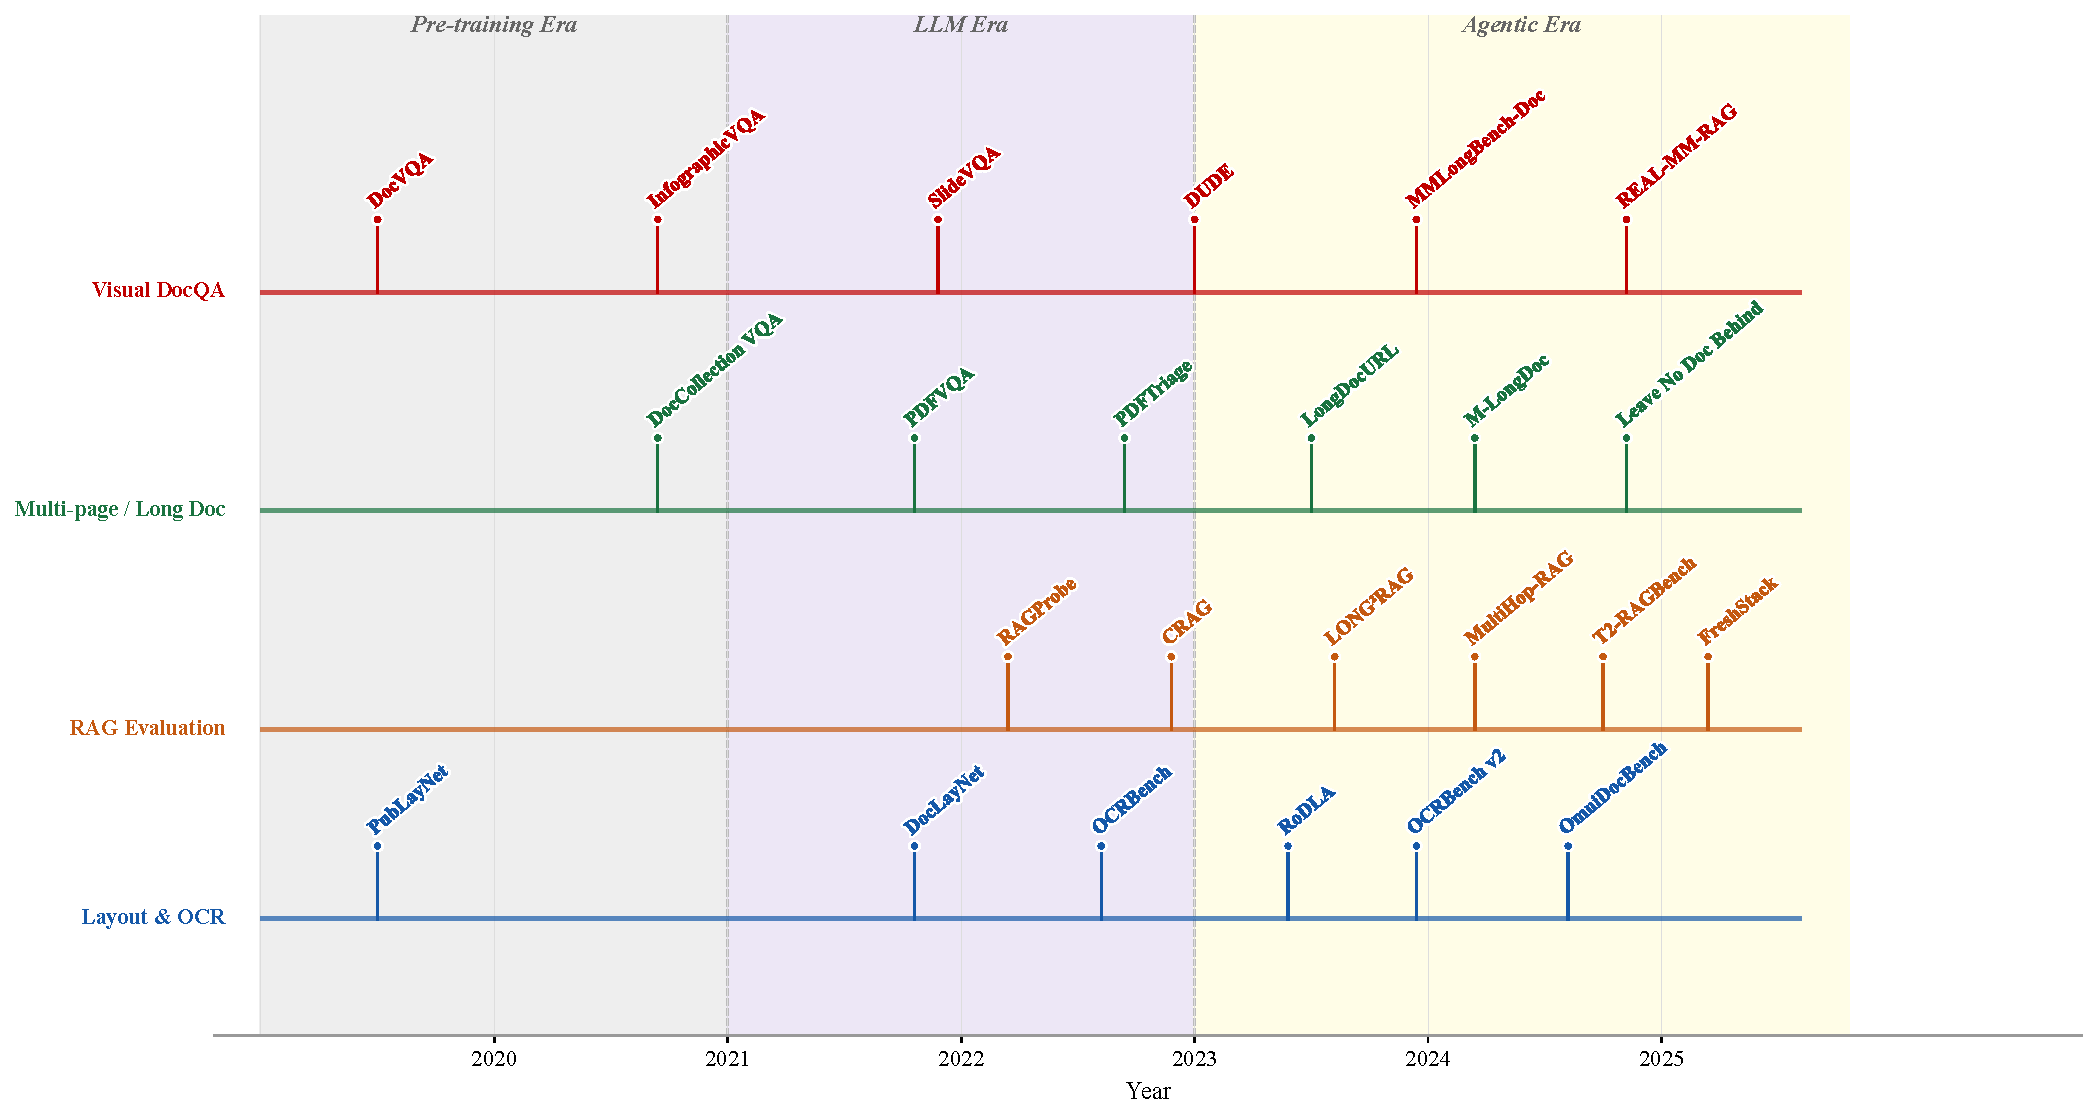
\includegraphics[
    width=0.95\textwidth,
    trim=0cm 0cm 0cm 0cm,
    clip
]{figs_by_qixingyu/fig10.pdf}
\caption{Benchmark landscape for document intelligence (2019--2025): evaluation datasets are organized into four categories---visual document question answering, multi-page and long-document understanding, retrieval-augmented generation evaluation, and layout analysis with optical character recognition---arranged chronologically by year of publication.}
\label{fig:benchmarks}
\end{figure*}

\subsubsection{Document QA Evaluation}

The exploration of document evaluation truly oriented toward RAG appeared in the following stages. RAGProbe \cite{ragprobe2023} is a dataset for evaluating Retrieval-Augmented Generation, covering complex question forms in real products (multiple sub-questions, cross-document, unanswerable, etc.).

Next, a large body of work began to explicitly distinguish the four stages of retrieval / grounding / reasoning / generation and constructed explainable or controllable evaluation frameworks. General and systematic method evaluation benchmarks include the following works. CRAG \cite{crag2024} proposed designing a task set covering multiple domains, document structures, and question types, allowing researchers and engineers to compare different RAG architectures, retrievers, re-rankers, and generative models using the same data and metrics. Such a unified evaluation design allows RAG optimization to move from "subjective parameter tuning" to more quantifiable and reproducible experimental comparisons. Unanswerability Evaluation for RAG \cite{unanswerablerag2024} measures whether a system can correctly refuse to answer when encountering unanswerable queries in documents, systematically expanding "unanswerability" into fine-grained categories for the first time. LONG²RAG \cite{long2rag2024} is an evaluation benchmark for long-context, long-form RAG systems, used to systematically measure the real capabilities of large models in "reading long text, retrieving multiple documents, and generating long answers" scenarios. Fact, Fetch, and Reason \cite{factfetchreason2024} argued for measuring the overall performance of end-to-end systems in real application scenarios. Each sample is a multi-hop QA question where answers are often scattered across multiple Wikipedia articles, sometimes requiring numerical calculation (e.g., "how many times faster"), table queries, temporal reasoning, combining multiple conditions, or post-processing retrieval results.

Many datasets in Chinese and domain-specific directions have also emerged. CRUD-RAG \cite{crudrag2024} is a large-scale Chinese benchmark for RAG systems, abstracting four major application types from the classic CRUD operations of "user interaction with knowledge bases" to perform comprehensive end-to-end and component-level evaluation of RAG. LegalBench-RAG \cite{legalbenchragr2024} is an evaluation benchmark specifically for the "retrieval stage" in the legal domain, used to measure the precision retrieval capabilities of various retrievers on complex legal documents. OmniEval \cite{omnieval2024} is a comprehensive evaluation benchmark for financial RAG systems, used to automatically and comprehensively assess the retrieval and generation capabilities of financial RAG/Agent systems in real financial scenarios. RAGCare-QA \cite{ragcareqa2025}, carefully curated and human-annotated, is a medical RAG evaluation benchmark dataset for systematically evaluating RAG pipelines and model performance in "theoretical medical knowledge QA" scenarios. RAGPPI \cite{ragppi2024} is a RAG benchmark and evaluation framework for the Protein-Protein Interaction (PPI) field, used to evaluate the capability of large models to answer questions related to the biological impact of PPI in drug target discovery scenarios.

Simultaneously, document and multi-modal long-context benchmarks matured rapidly. M3DocVQA \cite{m3docvqa2024} is an open-domain, multi-page, multi-document DocVQA benchmark dataset, primarily serving DocVQA/RAG research for multimodal retrieval and large models. MMLongBench-Doc \cite{mmlongbenchdoc2024} is a benchmark dataset and evaluation framework for multimodal long-context document understanding, mainly used to test the reading comprehension, retrieval, and reasoning capabilities of LVLMs in real long-document PDF scenarios. MMDocBench \cite{mmdocbench2024} is similarly a benchmark and framework for multimodal long-context understanding to test LVLMs in real PDF scenarios. DOCBENCH \cite{docbench2024} is an evaluation benchmark for LLM document reading systems, used to systematically assess the end-to-end capabilities of document reading systems in real interaction scenarios involving "uploading raw documents + asking questions about them." LongDocURL \cite{longdocurl2024} is a large-scale evaluation dataset for long-form multimodal document understanding, used to systematically evaluate the capabilities of multimodal large models in long document understanding, numerical reasoning, and cross-element localization. It focuses on complex PDF documents of dozens or even hundreds of pages, dividing tasks into three main categories: Understanding (U), Reasoning (R), and Locating (L). M-Longdoc \cite{mlongdoc2024} is an evaluation benchmark and framework for "multimodal ultra-long document understanding," used to systematically evaluate and improve the QA and reasoning capabilities of LVLMs/LMMs on hundreds of pages of documents. Proposed in 2024, it focuses on ultra-long PDF documents in realistic scenarios, emphasizing open-ended answering and retrieval augmentation. Leave No Document Behind \cite{leavenodocumentbehind2024} proposed a long-context LLM evaluation benchmark to systematically test models' long-context understanding in "extended multi-document QA" scenarios, defining four types of tasks: Spotlight Locating, Comparison, Clustering, and Chain of Reasoning.

\subsubsection{Real-World Image-Text Interaction Document Evaluation}

As research progresses toward real-world settings, most recent datasets involve image-text interaction. REAL-MM-RAG \cite{realmmrag2025} focuses on real enterprise/document scenarios, emphasizing "difficult retrieval and high robustness" across multiple modalities such as text, tables, and images. CRAG-MM \cite{cragmm2024} is a comprehensive RAG evaluation benchmark for multi-modal, multi-person multi-turn dialogue scenarios, mainly focusing on the real application scenario of "wearable devices + visual QA + retrieval augmentation." Visual-RAG \cite{visualrag2025} is a benchmark and evaluation framework for text-to-image RAG, containing numerous visual knowledge-intensive questions and related image candidate sets. Seeing Through the MiRAGE \cite{mirage2025} is an evaluation framework and benchmark for multimodal RAG, specifically designed to measure the factuality and citation quality of models when retrieving, generating, and citing from multimodal sources such as text, images, audio, and video. UNIDOC-BENCH \cite{unidocbench2025} extracts pages from real enterprise-level PDFs, annotating text blocks, tables, and images with evidence links, and then automatically or semi-automatically constructs multimodal QA pairs. Questions cover four typical RAG tasks: factual retrieval, comparison, summarization, and logical reasoning. VisR-Bench \cite{visrbench2025} proposed a multi-lingual long-document visual retrieval benchmark for visual RAG, focusing on the complete workflow of "retrieving the appropriate page from long multi-page documents and then answering." Benchmarking Retrieval-Augmented Multimodal Generation for Document QA \cite{benchmarkmmrag2025} focuses on mixed image-text information in real complex documents (long PDFs, reports, papers, etc.), including text, formulas, charts, tables, infographics, etc., with complex layouts. Each sample consists of a question, a short answer, and an evidence chain with layout positions. Retrieval for multi-hop and complex reasoning is also gradually developing. MultiHop-RAG \cite{multihoprag2024} is a benchmark and evaluation suite for multi-hop RAG, used to systematically evaluate the retrieval and reasoning capabilities of RAG in complex multi-hop QA scenarios. DocHop-QA \cite{dochopqa2025} focuses on real-world "cross-document, multi-structure, multi-step reasoning" complex information retrieval and reasoning scenarios. Automatically constructed from scientific PDF documents, questions often require aggregating evidence across multiple documents, pages, and structural blocks (paragraphs, tables, captions, etc.) to get the answer, rather than direct lookup in a single text segment. FanOutQA \cite{fanoutqa2024} focuses on so-called "fan-out" questions: one question requires simultaneously finding and integrating information across numerous entities and multiple documents. MHTS \cite{mhts2025} proposed systematically controlling reasoning difficulty to construct high-quality, diverse, and adjustable-difficulty multi-hop QA benchmarks for finer evaluation of RAG retrieval and generation.

RAG evaluation based on structured heterogeneous datasets is also receiving increasing attention. RAG over Tables \cite{ragovertables2025} refers to a set of evaluation benchmarks and frameworks proposed around RAG tasks on tabular data, oriented toward multi-table QA and RAG model evaluation on large-scale tabular corpora. T2-RAGBench \cite{t2ragbench2025} is a text-table hybrid RAG evaluation benchmark for the financial domain, used to systematically assess the model's capability in the complete "retrieval followed by numerical reasoning" process. mmRAG \cite{mmrag2025} is a modular benchmark for heterogeneous/multimodal RAG systems, using a unified framework to evaluate the retrieval and generation capabilities of systems across multiple knowledge sources like text, tables, and knowledge graphs. RAG-based QA over Heterogeneous Data and Text \cite{raghetero2024} is a set of research and experimental configurations around the QUASAR system for evaluating RAG QA capabilities on heterogeneous data sources. Dynamic RAG evaluation datasets based on time have also been proposed. DRAGON \cite{dragon2024} is a dynamic RAG evaluation benchmark for news scenarios, mainly focusing on systematically evaluating the retrieval and generation capabilities of RAG on continuously changing news corpora in a Russian environment. FreshStack \cite{freshstack2025} is an evaluation benchmark and construction framework for technical document retrieval/RAG systems, specifically designed to evaluate the real performance of technical document retrieval and technical RAG QA in 2025 and beyond. It automatically constructs datasets from real community QA, focusing on rapidly evolving and easily contaminated technical fields.

Long-context and retrieval-free control evaluations were subsequently proposed. LaRA \cite{lara2025} focuses on evaluating whether LLMs in typical 2025 applications should rely more on ultra-long context input or obtain information through external retrieval. Ko-LongRAG \cite{kolongrag2025} is an evaluation benchmark specifically for Korean long-context RAG. It simulates real long-document retrieval scenarios through a "retrieval-free construction method" to systematically evaluate various large models on Korean long-context RAG tasks. Summary of a Haystack \cite{summaryhaystack2024} is an evaluation benchmark for long-context large models and RAG systems, focusing on testing the system's robust long-text understanding and aggregation capabilities in million-token contexts. Proposed in 2024, it emphasizes "finding and correctly summarizing important content" in complex multi-document scenarios. Are We on the Right Way for Assessing Document RAG? \cite{rightwaydocumentrag2025} is a systematic analysis and benchmark design study on document-level RAG evaluation methods. It focuses on the deficiencies of current document RAG benchmarks and proposes a new evaluation system, Double-Bench, as an alternative.

In addition to benchmarks directly oriented toward RAG, a series of document visual understanding datasets have systematically characterized the complexity of real documents at visual, structural, and linguistic levels in parallel evolution. These benchmarks do not directly evaluate the retrieval or generation performance of RAG but define the upper limit of input difficulty and the perceptual prerequisites that RAG systems must face in real document scenarios. These include RoDLA \cite{rodla2024}, a robustness benchmark for document layout analysis. It systematically evaluates the stability of layout detection/segmentation model performance under real interference conditions, making it an important robustness evaluation benchmark in the current DLA field. U-DIADS-Bib \cite{udiadsbib2024} is a document layout analysis benchmark for ancient manuscripts, focusing on pixel-level semantic layout segmentation to evaluate and drive algorithm development for tasks such as codex layout understanding, OCR preprocessing, and automatic transcription. M6Doc \cite{m6doc2023} is an open dataset for modern document layout analysis, particularly emphasizing real scenarios, multiple formats, multiple languages, and complex layouts, significantly impacting document understanding and OCR preprocessing. MosaicDoc \cite{mosaicdoc2025} is a large-scale Chinese-English bilingual benchmark for visually rich document understanding, collecting images from newspapers and magazines, containing highly heterogeneous visual elements such as illustrations, titles, subtitles, columns, and advertisement blocks. HW-MLVQA \cite{hwmlvqa2025} is a visual QA dataset and benchmark for multilingual handwritten document understanding, used to evaluate and drive the cross-modal and cross-lingual understanding capabilities of models on real handwritten documents. MTVQA \cite{mtvqa2025} is a benchmark for multilingual text-centric visual QA, used to systematically assess the capabilities of multimodal large models in multilingual scene text understanding and QA. All images come from real-world "text-rich scenes," covering over 20 scene types such as posters, signboards, document screenshots, product packaging, and interface screenshots. IconQA \cite{iconqa2024} is a large-scale visual QA dataset for "diagram reasoning," focusing on iconic scenarios such as abstract charts and textbook illustrations rather than natural images. A Comparative Review \cite{vdureview2025} is a survey work that systematically reviews the evolution of visual document understanding from traditional methods to deep learning and then to multimodal Transformers in recent years. It points out that real-world documents such as invoices, receipts, tables, research reports, and questionnaires contain text, layout, and visual elements simultaneously, thus requiring a concentrated, comparative review for visual document understanding. Together, these works constitute the perceptual and structural foundation for document-level and multimodal RAG systems, explaining why RAG performance in real-world documents is often limited by input parsing and evidence structuring capabilities rather than just the retrieval or generation modules themselves.